
\begin{table*}[t]
\centering
\setlength{\tabcolsep}{7pt}
\renewcommand{\arraystretch}{0.85}
\caption{
当初始学生-教师重叠比率较低时，Semi-OPD优于其他OPD变体，而在比率较高时仍保持相当的性能。  
结果以温度为1.0时的avg@32报告，对60/80/100步的检查点进行平均。$^\S$ 来自~\citep{xu2026pass}。
}
\begin{tabular}{lccccc}
\toprule
Method
& AIME24 & AIME25 & AIME26 & HMMT Feb26 & Avg@32 \\
\midrule

\multicolumn{6}{l}{
\textbf{Qwen3-1.7B (Non-think) $\leftarrow$ Qwen3-4B-Instruct-2507 }
\hfill {\normalfont \underline{Initial overlap ratio: 62.5\%}}
} \\
\addlinespace[2pt]

\textit{Teacher}
& 60.4 & 46.0 & 52.2 & 31.2 & 47.5 \\
\textit{Student, untrained}
& 12.6 & 9.6 & 7.4 & 6.3 & 9.0 \\

\addlinespace[1pt]
Standard OPD$^\S$
& 35.8 & 25.5 & 23.3 & 20.1 & 26.2 \\
Speculative KD~\citep{xuspeculative}$^\S$
& 33.1 & 30.7 & 28.9 & 20.1 & 28.2 \\
FastOPD~\citep{zhang2026fast}$^\S$
& 42.3 & 30.4 & 26.4 & 23.6 & 30.7 \\
Lightning OPD~\citep{wu2026lightning}
& 41.0 & 28.8 & 27.5 & 22.7 & 30.0 \\
Relay-OPD~\citep{xu2026pass}$^\S$
& 42.7 & 32.8 & 30.5 & 24.7 & 32.7 \\
\textbf{\method (ours)}
& \textbf{50.3}
& \textbf{38.9}
& \textbf{41.8}
& \textbf{28.0}
& \textbf{39.8} \\


\midrule

\multicolumn{6}{l}{
\textbf{Qwen3-4B (Non-think) $\leftarrow$ Qwen3-30B-A3B-Instruct-2507}
\hfill {\normalfont \underline{Initial overlap ratio: 62.5\%}}
} \\
\addlinespace[2pt]

\textit{Teacher}
& 72.9 & 62.0 & 72.8 & 40.6 & 62.1 \\
\textit{Student, untrained}
& 23.6 & 18.0 & 16.8 & 14.9 & 18.3 \\

\addlinespace[1pt]
Standard OPD
& 55.1 & 45.3 & 49.1 & 30.0 & 44.9 \\
FastOPD~\citep{zhang2026fast}
& 63.5 & 55.5 & 56.2 & 34.9 & 52.5 \\
Lightning OPD~\citep{wu2026lightning}
& 64.0 & 56.8 & 54.3 & 33.5 & 52.2 \\
Relay-OPD~\citep{xu2026pass}
& 61.1 & 48.1 & 52.5 & 32.8 & 48.6 \\
\textbf{\method (ours)}
& \textbf{66.4}
& \textbf{63.1}
& \textbf{62.9}
& \textbf{37.4}
& \textbf{57.4} \\


\midrule







\multicolumn{6}{l}{
\textbf{NM-Cascade-2-30B-A3B $\leftarrow$ NM-Cascade-2-Math-Expert}
\hfill {\normalfont \underline{Initial overlap ratio: 89.3\%}}
} \\
\addlinespace[2pt]

\textit{Teacher}
& 82.8 & 80.0 & 76.4 & 58.2 & 74.4 \\
\textit{Student, untrained}
& 77.9 & 72.4 & 68.8 & 49.3 & 67.1 \\

\addlinespace[1pt]
Standard OPD
& 83.0 & 80.1 & 75.8 & 57.5 & 74.1 \\
FastOPD~\citep{zhang2026fast}
& 83.0 & \textbf{80.7} & \textbf{77.1} & \textbf{58.4} & \textbf{74.8} \\
Lightning OPD~\citep{wu2026lightning}
& \textbf{83.2} & 79.1 & 75.7 & 56.8 & 73.7 \\
Relay-OPD~\citep{xu2026pass}
& \textbf{83.2} & 80.1 & 73.3 & 57.7 & 73.6 \\
\textbf{\method (ours)}
& 83.0 & 79.7 & 77.0 & 56.8 & 74.1 \\

\bottomrule
\end{tabular}
\label{tab:baselines}
\vspace{-0.5em}
\end{table*}




\subsection{半OPD与OPD及其变体的基准测试}
\label{sec:experiments}
\vspace{-2mm}












\noindent \textbf{实验设置。}
我们在17组学生-教师模型对（完整的模型对名称见附录中的表~\ref{tab:allpairs}）上进行实验，涵盖Qwen3~\citep{qwen3}、DeepSeek-R1-Distill~\citep{deepseekai2025deepseekr1incentivizingreasoningcapability}和Nemotron-Cascade-2~\citep{yang2026nemotron}系列。Qwen3的学生模型（1.7B、4B和14B）从Instruct和Thinking教师模型中蒸馏而来，教师模型参数规模最高达235B-A22B，使用原始初始化或SFT预热初始化；DeepSeek-R1-Distill的学生模型（1.5B和7B）则从同一检查点的强化学习训练后代中蒸馏而来，包括JustRL~\citep{he2025justrl}、Polaris~\citep{Polaris2025}、Light-R1~\citep{lightr1proj}和DeepCoder~\citep{deepcoder2025}；而Nemotron-Cascade-2模型对由OPD步骤前的学生检查点及其用于OPD步骤的数学领域教师模型组成~\citep{yang2026nemotron}。这些模型对覆盖了非思考模式与思考模式，每组内的训练与评估均保持一致。所有模型均在DAPO-Math~\citep{yu2025dapo}上进行蒸馏。数学能力通过在AIME 2024--2026和HMMT February 2026上的$\mathrm{avg}@32$准确率来衡量，评估回放限制在32k token以内（Nemotron-Cascade-2为40k），跨领域泛化能力则在HumanEval和HumanEval+~\citep{chen2021evaluating}上评估。更多细节见附录~\ref{app:setup}。





\begin{figure*}[t]
  \centering
  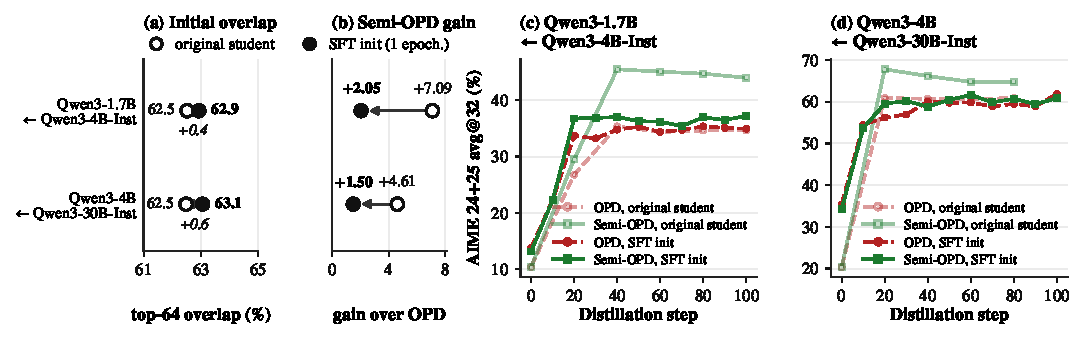
\includegraphics[width=\linewidth]{figures/fig_sft.pdf}
\vspace{-1.5em}
\caption{
\textbf{教师回放SFT提升了重叠率，但在半监督OPD后降低了最终性能。} \textbf{(a)} 在教师回放上进行SFT略微提高了初始的前64重叠率。 \textbf{(b)} 在教师回放上进行SFT后再进行半监督OPD，仍优于OPD，但表现不如仅使用半监督OPD。 \textbf{(c, d)} 在教师回放上进行SFT与半监督OPD结合后，对最终性能产生了负面影响。
}

  \label{fig:sft}
  \vspace{-1em}
\end{figure*}




\textbf{Semi-OPD 与 OPD 在 17 组模型对上的对比。} 图~\ref{fig:allpairs} 展示了在所有 17 组教师-学生模型对上，Semi-OPD 和 OPD 在训练过程中达到的平均准确率演化情况。我们按照初始教师-学生模型对的重叠比例对这些模型对进行排序，该比例标注在每个图表上方。此外，我们报告了 Semi-OPD 相对于 OPD 的平均准确率提升，其定义为 Semi-OPD 与 OPD 学习曲线之间的面积除以它们共享的训练周期。


我们观察到，在17对中的14对上，Semi-OPD的表现优于OPD，其在最后一步的提升最高可达$\sim$ 13\%，且在初始重叠度较低的配对上通常取得最大增益。在其余三对上，Semi-OPD仍能实现相当的性能，差距仅为0.1--2.6\%。对于Qwen3思考模式的配对，这种差异尤为明显：OPD在训练过程中出现显著的性能下降，而Semi-OPD则持续提升。




\noindent \textbf{与OPD变体在准确率和训练效率上的比较。} 除了标准OPD外，我们还针对三种不同模型大小、重叠比率和推理模式的模型对，将Semi-OPD与近期的OPD变体进行了对比，如表~\ref{tab:baselines}所示。我们观察到：(1) 在Qwen3-1.7B（非思考）和Qwen3-4B（非思考）学生模型上，其师生重叠比率较低，Semi-OPD在准确率方面优于所有其他基准方法，同时训练效率最高，例如，在这两个模型对上分别比Relay-OPD高出7.1\%和8.8\%的准确率，且训练时间分别减少了35$\times$和19.5$\times$，如图~\ref{fig:speedup}和表~\ref{tab:speedup}所示。(2) 在Nemotron-Cascade-2模型对上，其重叠比率约为89\%，我们的Semi-OPD仍与其他OPD基准方法保持竞争力，仅以0.7\%的准确率差距略逊于最佳基准，同时相比FastOPD将训练时间减少2.2倍，相比OPD减少4.5倍。

总体准确率-训练效率权衡如图~\ref{fig:speedup}所示，其中Semi-OPD相较于标准OPD实现了高达11.4$\times$的加速，相较于最快的基准方法FastOPD也实现了2.7$\times$的加速。相比之下，另一种OPD变体Relay-OPD虽然同样旨在使学生模型的生成更接近教师模型，但需要交替进行教师和学生的生成，导致效率较低。







